\chapter{Sviluppi tecnologici}\label{ch:sviluppi}
Questo capitolo riguarda i miglioramenti realizzati dal punto di vista tecnologico che sono andati direttamente ad impattare la piattaforma AirQino, migliorandone in un caso l'affidabilità dei dati e nell'altro i tempi di risposta del database per query particolarmente onerose.

% Replica del database di produzione
\section{Replica del database di produzione}\label{sec:replica}

Spesso fare analisi mediamente complesse sui dati contenuti in un database può comportare rallentamenti nei tempi di risposta. Se questi carichi risultano frequenti, il sistema può arrivare a bloccarsi e provocare interruzioni del servizio.

Una soluzione per risolvere questo problema è la creazione di una (o più) repliche del database primario. Nella replica, i dati e gli oggetti del database vengono copiati e distribuiti su un altro spazio fisico. Le operazioni onerose a questo punto possono essere fatte direttamente sulla replica che agisce come nodo secondario: in questo modo, il carico viene distribuito e non si intaccano le performance del database principale.

Il concetto di \textit{replica} è diverso dal \textit{mirroring}, in cui vengono create una o più copie di un database su diverse istanze del server, e funzionano come copie di riserva (e si attivano soltanto nel caso di guasto del nodo principale).

Un sistema di replica correttamente implementato può offrire diversi vantaggi, tra cui riduzione del carico (perchè i dati replicati possono essere distribuiti su più server), efficienza (i server offrono prestazioni migliori perchè meno gravati da query pesanti) e ridondanza (i dati sono raggiungibili da più indirizzi).

Di contro, questa tecnica comporta la necessità di mantenimento dei nodi secondari, spesso collocati su server diversi (con i costi a questi associati). Inoltre, repliche errate o non implementate in maniera corretta possono causare la mancata sincronizzazione tra i nodi, portando ad una perdita o incoerenza dei dati.

\subsection{Motivazioni}\label{ssec:replica-motivazioni}
L'affidabilità dei dati rappresenta uno dei punti critici per un sistema di ingestione di grosse quantità di dati. Questo è vero anche caso di AirQino, dove infatti il database di produzione conta oltre 100 milioni di misurazioni rilevate, in continuo aumento con una media di 300 inserimenti al minuto.

La replica offrire vantaggi in questo senso, principalmente legati alle prestazioni, disponibilità e sicurezza dei dati:
\begin{enumerate}
  \item \textbf{Maggiore affidabilità}: tramite la replica del database viene garantita la disponibilità dei dati anche nel caso in cui una delle macchine presenti un guasto hardware. In questo caso, il sistema di gestione del database distribuito deve essere in grado di indirizzare gli utenti interessati ad uno degli altri nodi disponibili;
  \item \textbf{Miglioramento delle prestazioni}: essendo i dati distribuiti su diverse istanze, accessi multipli non saturano i server. Questo aspetto risulta particolarmente importante per applicazioni che possono avere una grande quantità di richieste simultanee;
  \item \textbf{Maggiore sicurezza dei dati}: Mentre in un sistema tradizionale i backup di un database (se effttuati) sono archiviati sullo stesso disco, con la replica del database vengono scritti su più server, aumentandone di fatto l'affidabilità e la ridondanza.
\end{enumerate}

Esistono diverse tecniche di replicazione del database, che dipendono sia dalla tecnologia utilizzata (MySQL, Postgres) che dalla natura del database stesso (relazionale o non relazionale). Il database di AirQino fa uso di Timescale\footnote{Timescale: Time-series data simplified - \url{https://www.timescale.com}}, basato su Postgres; una caratteristica di Postgres è la possibilità di replicazione con la tecnologia di \textbf{Streaming Replication}, descritta di seguito.

\subsection{Streaming replication}\label{ssec:streaming-replication}
La streaming replication di PostgreSQL è una funzionalità che consente di replicare i dati in tempo reale da una istanza di PostgreSQL a un'altra. Questo significa che, se si modificano i dati in una delle istanze, questi saranno immediatamente replicati anche nell'altra istanza. Questa istanza database di replica di lettura ("standby" in termini PostgreSQL) è una replica fisica creata in modo asincrono dell'istanza del database primario.

PostgreSQL fa utilizza un \textit{ruolo di replica} (\textit{replication role}) per eseguire la replica in streaming (il ruolo presenta dei privilegi ma non può essere utilizzato per modificare i dati, la replica infatti è di sola lettura).

La replica si basa sulle transazioni \textbf{WAL} (Write Ahead Log) e utilizza il protocollo TCP per garantire una connessione sicura tra i server e inviare in modo asincrono le modifiche al database via via che vengono effettuate.

È possibile promuovere una replica di lettura PostgreSQL a una nuova istanza database di origine. Una volta promossa, la replica smette di ricevere comunicazioni WAL e non è più un'istanza di sola lettura.

PostgreSQL salva le informazioni aggiornate del server primario in registro delle transazioni, noto come registro \textit{write-ahead}, utile in preparazione per il ripristino dopo un'interruzione o per un \textit{rollback}. La replica in streaming funziona proprio trasferendo e applicando il WAL al server di replica in tempo reale.

\begin{figure}[H]
\centering
\captionsetup{justification=centering}
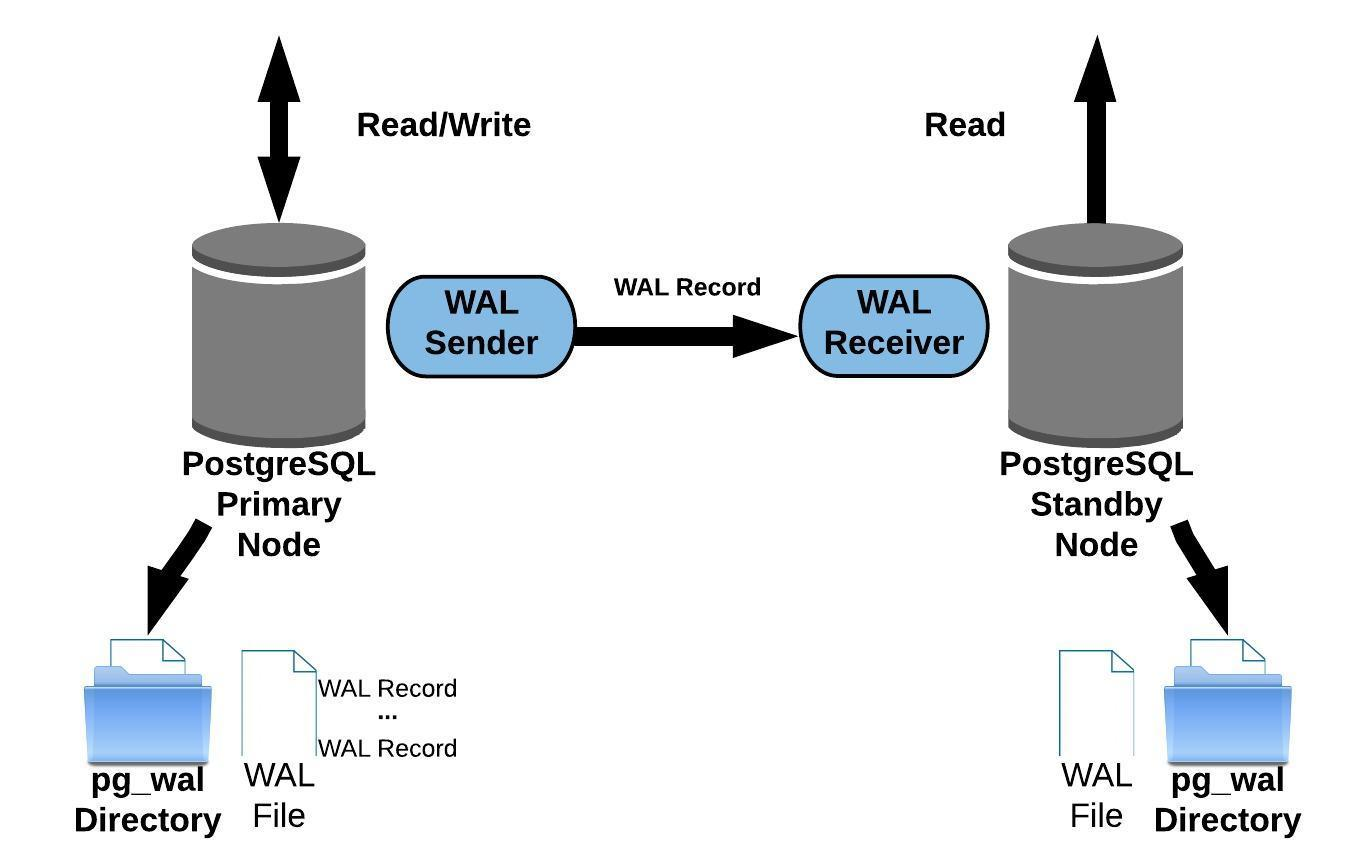
\includegraphics[width=0.75\textwidth,height=\textheight,keepaspectratio]{img/streaming_replication.jpg}
\caption{Streaming Replication di PostgreSQL\\Fonte: \url{https://severalnines.com}}
\label{fig:streaming-replication}
\end{figure}

La replica in streaming può essere costruita in una configurazione 1:N, con un solo server primario, ma è possibile anche aggiungere più server di replica (configurazione \textit{multi-standby}). È anche possibile realizzare una configurazione a cascata, in cui un server di replica si connette ad un altro server di replica.

Per la replica in streaming, è possibile scegliere se effettuare una modalità sincrona oppure asincrona. La differenza tra replica sincrona e replica asincrona sta nell'attesa o meno della risposta dal server di replica prima di completare l'elaborazione sul server primario:
\begin{itemize}
  \item \textbf{Replica sincrona}: il server primario attende una risposta dal server di replica prima di completare un processo. In questo caso il tempo di risposta complessivo include anche il tempo di spedizione del registro;
  \item \textbf{Replica asincrona} (impostazione predefinita): il server primario completa un processo senza attendere una risposta dal server di standby. Pertanto, il tempo di risposta complessivo è praticamente lo stesso di quando non viene utilizzata la replica in streaming; in questa modalità il risultato aggiornato sul server primario potrebbe non essere immediatamente disponibile sul server di replica. \cite{streaming_replication}
\end{itemize}

Ci sono però alcune limitazioni nell'utilizzo di repliche con PostgreSQL:
\begin{itemize}
  \item Ogni replica di lettura PostgreSQL è di sola lettura. Non è possibile creare una replica di lettura che sia anche scrivibile;
  \item Non è possibile creare una replica di lettura da un'altra replica di lettura a cascata;
  \item Gli utenti e i ruoli di accesso vengono rispecchiati dall'istanza primaria, il che significa che non è possibile utilizzare credenziali diverse o aggiungere utenti aggiuntivi soltanto alla replica;
  \item Non è possibile creare tabelle e viste nell'istanza di replica; in pratica si possono solo eseguire query di tipo \textit{SELECT}.
\end{itemize}

La sezioni seguenti spiegano il lavoro svolto per configurare la replica del database di produzione della piattaforma AirQino.

\subsubsection{Preparazione del database primario}

\begin{enumerate}
  \item Per avviare la procedura, è stato sul database un utente PostgreSQL con un ruolo adatto ad avviare la \textit{streaming replication} con il comando SQL:
  \vspace{1mm}
   \begin{lstlisting}[language=sql]
SET password_encryption = 'scram-sha-256'; 
CREATE ROLE repuser WITH REPLICATION PASSWORD 'SOME_SECURE_PASSWORD' LOGIN;\end{lstlisting}
  \item Sono stati poi aggiunti i seguenti parametri di configurazione al file \url{/var/lib/postgresql/data/postgresql.conf}:
  \vspace{1mm}
  \begin{lstlisting}[]
listen_addresses= '*'
wal_level = replica
max_wal_senders = 2
max_replication_slots = 2
synchronous_commit = off
\end{lstlisting}

  \item Sono stati inoltre aggiunti i seguenti parametri al secondo file di configurazione \url{/var/lib/postgresql/data/pg_hba.conf} per configurare l'autenticazione basata su host in modo da accettare connessioni dalla replica\footnote{Dalla documentazione Streaming Replication: \url{https://www.postgresql.org/docs/current/warm-standby.html\#STREAMING-REPLICATION}}:
  \vspace{1mm}
\begin{lstlisting}[]
host     replication     repuser   <REPLICA_IP>/32       scram-sha-256
\end{lstlisting}
dove \textit{repuser} è l'utente creato al passo 1 e \textit{REPLICA\_IP} è l'IP della macchina in cui si trova la replica;
  \item È stato riavviato il database per applicare i cambiamenti;
  \item Infine è stato creato uno slot di replicazione sul database con il comando SQL:
  \vspace{1mm}
  \begin{lstlisting}[language=sql]
SELECT * FROM pg_create_physical_replication_slot('replica_1_slot');
\end{lstlisting}
\end{enumerate}

\subsubsection{Configurazione della replica}
Di seguito sono elencati i passi eseguiti per configurare la replica:

\begin{enumerate}
  \item È stata interrotta l'istanza Postgres:
  \vspace{1mm}
\begin{lstlisting}[]
pg_ctl -D $PGDATA -m fast -w stop
\end{lstlisting}
  \item Sono stati cancellati i contenuti della cartella \textit{PGDATA}:
  \vspace{1mm}
\begin{lstlisting}[]
rm -rf $PGDATA/*
\end{lstlisting}
  \item È stato avviato il backup del database primario:
  \vspace{1mm}
\begin{lstlisting}[]
pg_basebackup -h <PRIMARY_HOST> -p <PRIMARY_PORT> -D $PGDATA -U repuser -vP -R -W
\end{lstlisting}
Dove \textit{PRIMARY\_HOST} è l'IP della macchina in cui si trova il database primario, \textit{PRIMARY\_PORT} è la porta del database primario e \textit{repuser} è l'utente di replicazione creato al passo 1.

Da notare che con la flag \textit{-W} viene chiesta in maniera interattiva la password di replicazione, impostata in precedenza (\textit{SOME\_SECURE\_PASSWORD});
  \item Infine è stata avviata l'istanza Postgres:
  \vspace{1mm}
\begin{lstlisting}[]
pg_ctl -D $PGDATA -w start
\end{lstlisting}
A questo punto la replica è attiva e sincronizzata 1:1 in tempo reale con il database primario.
\end{enumerate}

\subsubsection{Automazione con Docker}
L'intero setup (sia database primario che la replica) può essere automatizzato con Docker e docker-compose, in modo da far partire la sincronizzazione direttamente all'avvio del container.
Poichè i passi per creare la replica richiedono di stoppare l'istanza Postgres, questa procedura non si può eseguire all'interno del container Docker stesso, già avviato, perchè si andrebbe a stoppare tutto il container.
Per questo è necessario dare i comandi per la replica da uno script di \textit{entrypoint} che viene eseguito subito prima di avviare il container:
\begin{enumerate}
  \item È stato creato un \url{Dockerfile} da immagine Timescale (\url{timescaledb:latest}), con l'aggiunta di uno script \textit{entrypoint}, così strutturato:
  \vspace{1mm}
  \begin{lstlisting}[]
FROM timescale/timescaledb:latest-pg13
ADD replica.sh /docker-entrypoint-initdb.d/
\end{lstlisting}
  \item È stato creato il file \url{replica.sh} che verrà eseguito tutte le volte che si avvia il database, con il seguente contenuto:
  \vspace{1mm}
  \begin{lstlisting}[]
echo "Stopping Postgres instance..." 
pg_ctl -D ${PGDATA} -m fast -w stop

echo "Clearing PGDATA folder..." 
rm -rf ${PGDATA}

echo "Creating base backup..." 
PGPASSWORD=${REPLICATION_PASSWORD} pg_basebackup -h ${REPLICATION_HOST} -p ${REPLICATION_PORT} -D ${PGDATA} -U ${REPLICATION_USER} -vP -R -w

echo "Restarting Postgres instance..." 
pg_ctl -D ${PGDATA} -w start
\end{lstlisting}
Come già accennato, la flag \textit{-W} di \textit{pg\_basebackup} chiede la password in maniera interattiva, ma questo ovviamente non è adatto a script automatizzati che invece non richiedono interazione. Come alternativa è stata utilizzata la flag \textit{-w} (minuscola) e passata la password come variabile di ambiente chiamata \textit{PGPASSWORD};
\item È stato creato il file \url{docker-compose.yml} così strutturato (ridotto per semplicità):
\vspace{1mm}
  \begin{lstlisting}[]
services:
  replica:
    build:
        context: .
        dockerfile: Dockerfile
    environment:
        # Cartella PDATA custom
        PGDATA: /var/lib/postgresql/data/pgdata

        # Parametri di replicazione
        REPLICA_USER: repuser # Utente di replicazione impostato al punto 1
        REPLICATION_HOST: x.x.x.x # IP del db primario
        REPLICATION_PORT: x # Porta del db primario
        REPLICATION_PASSWORD: SOME_SECURE_PASSWORD # Password di replicazione impostata al punto 1
    ports:
        - 45432:5432
    volumes:
        - /var/replica-pg13-timescale/:/var/lib/postgresql/data
\end{lstlisting}

  \item Infine, è stato avviato il container con \url{docker-compose} \url{up}.
\end{enumerate}

In questo modo la replica viene sincronizzata con il database primario automaticamente all'avvio del container Docker.
Allo stesso modo è possibile automatizzare con Docker anche il setup su database primario.

% Ottimizzazione di query temporali
\section{Ottimizzazione di query temporali}\label{sec:cont-aggr}
Ci sono molti vantaggi nell'aggregazione di dati:
\begin{itemize}
  \item \textbf{Flessibilità}: aggregare dati in tempo reale in base a qualsiasi criterio desiderato;
  \item \textbf{Risparmio di tempo}: non è necessario eseguire query aggiuntive per ottenere informazioni aggregate in tempo reale;
  \item \textbf{Risparmio di spazio} i dati aggregati in tempo reale occupano meno spazio rispetto ai dati non aggregati.
\end{itemize}

I dati delle serie temporali tendono a crescere molto rapidamente, e grandi volumi di dati possono rallentare quando si eseguono query con lo scopo di aggregare i dati (ad esempio per generare report o riepiloghi sull'andamento o sui trend di crescita/decrescita).

Per garantire efficienza e scalabiità con questa tipologia di dati, si rende quindi necessario fare in modo che le query su dati temporali abbiano un tempo di risposta costante, indipendentemente dalla quantità di dati e senza gravare sul database.

\subsection{Motivazioni}\label{ssec:cont-aggr-motivazioni}
La piattaforma AirQino (vedi \ref{sec:airqino}) raccoglie dati emessi ogni minuto da decine di centraline in diverse località. Per memorizzare questi dati viene utilizzato un database Postgres con estensione Timescale, che offre delle funzionalità specifiche proprio per dati di tipo temporale.

Una delle funzionalità di AirQino consente di mostrare un grafico dell'andamento (su base media oraria) dell'ultima settimana per diverse grandezze (temperatura, umidità, \ce{CO2}, \ce{NO2}, \ce{PM_{2.5}}, \ce{PM_10} etc...), come mostrato in figura \ref{fig:airqino-temp}.

\begin{figure}[H]
\centering
\captionsetup{justification=centering}
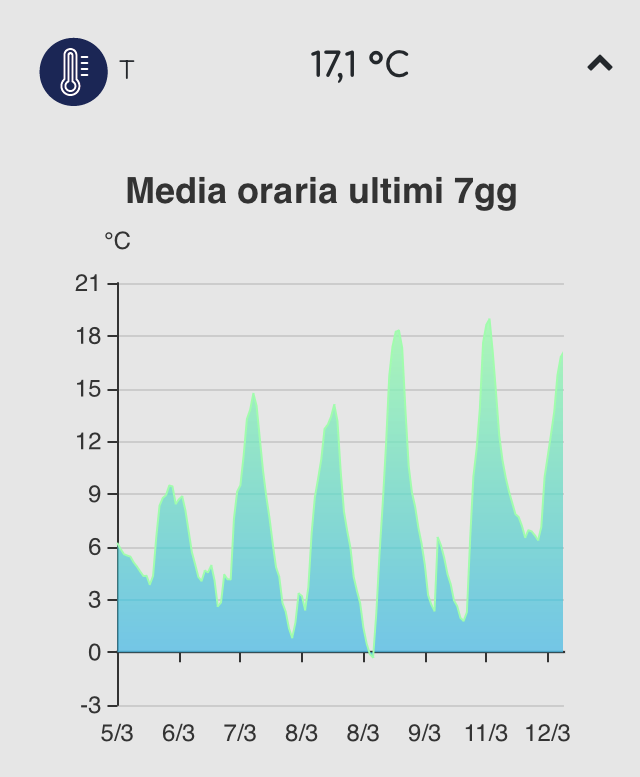
\includegraphics[width=0.45\textwidth,height=\textheight,keepaspectratio]{img/airqino_temp}
\caption{Grafico dell'andamento della temperatura nell'ultima settimana per una centralina AirQino.\\Fonte: \url{https://airqino.magentalab.it}}
\label{fig:airqino-temp}
\end{figure}

La piattaforma prevede inoltre altri casi d’uso per i dati a media oraria:
\begin{itemize}
  \item Visualizzazione sulla home page dell’applicazione le medie orarie degli ultimi 7 giorni;
  \item Esportazione dataset periodici, da mettere a disposizione degli utenti esterni (ad esempio pubbliche amministrazioni che hanno installato le centraline);
  \item Esportazione dataset \textit{on demand} da parte di utenti esterni, con indicazione di inizio/fine del periodo desiderato.
\end{itemize}
In tutti questi casi il requisito è di ottenere medie orarie del dato calibrato.

Per calcolare la media oraria nell'ultima settimana, ad ogni richiesta sul database viene eseguito una query SQL di questo tipo (ridotta per semplicità):

\vspace{1mm}
\begin{lstlisting}[language=sql]
SELECT time_bucket('1 hour', sd.data_acquired) as bucket, avg(sd.float_value)
FROM station_data sd
WHERE sd.data_acquired > NOW() - INTERVAL '7 days'
AND sd.sensor_id = 29510691 /* id centralina */
ORDER BY bucket DESC;
\end{lstlisting}

La query fa uso della funzione \textit{time\_bucket} di Timescale, che consente di partizionare la tabella con i dati dei sensori minuto per minuto direttamente in fasce orarie. L'utilizzo combinato con la funzione \textit{avg()} va poi a prendere la media del valore su tutta l'ora.

Questo però significa che se si desidera eseguire questa query più di una volta, il database deve eseguire la scansione dell'intera tabella e ricalcolare la media ogni volta. Nella maggior parte dei casi, tuttavia, i dati nella tabella non sono cambiati in modo significativo, quindi non è necessario eseguire la scansione dell'intero set di dati.

La figura \ref{fig:query-prima} mostra i tempi di risposta a questa query per tutte le centraline AirQino prima di aver applicato l'ottimizzazione.

\begin{figure}[H]
\centering
\captionsetup{justification=centering}
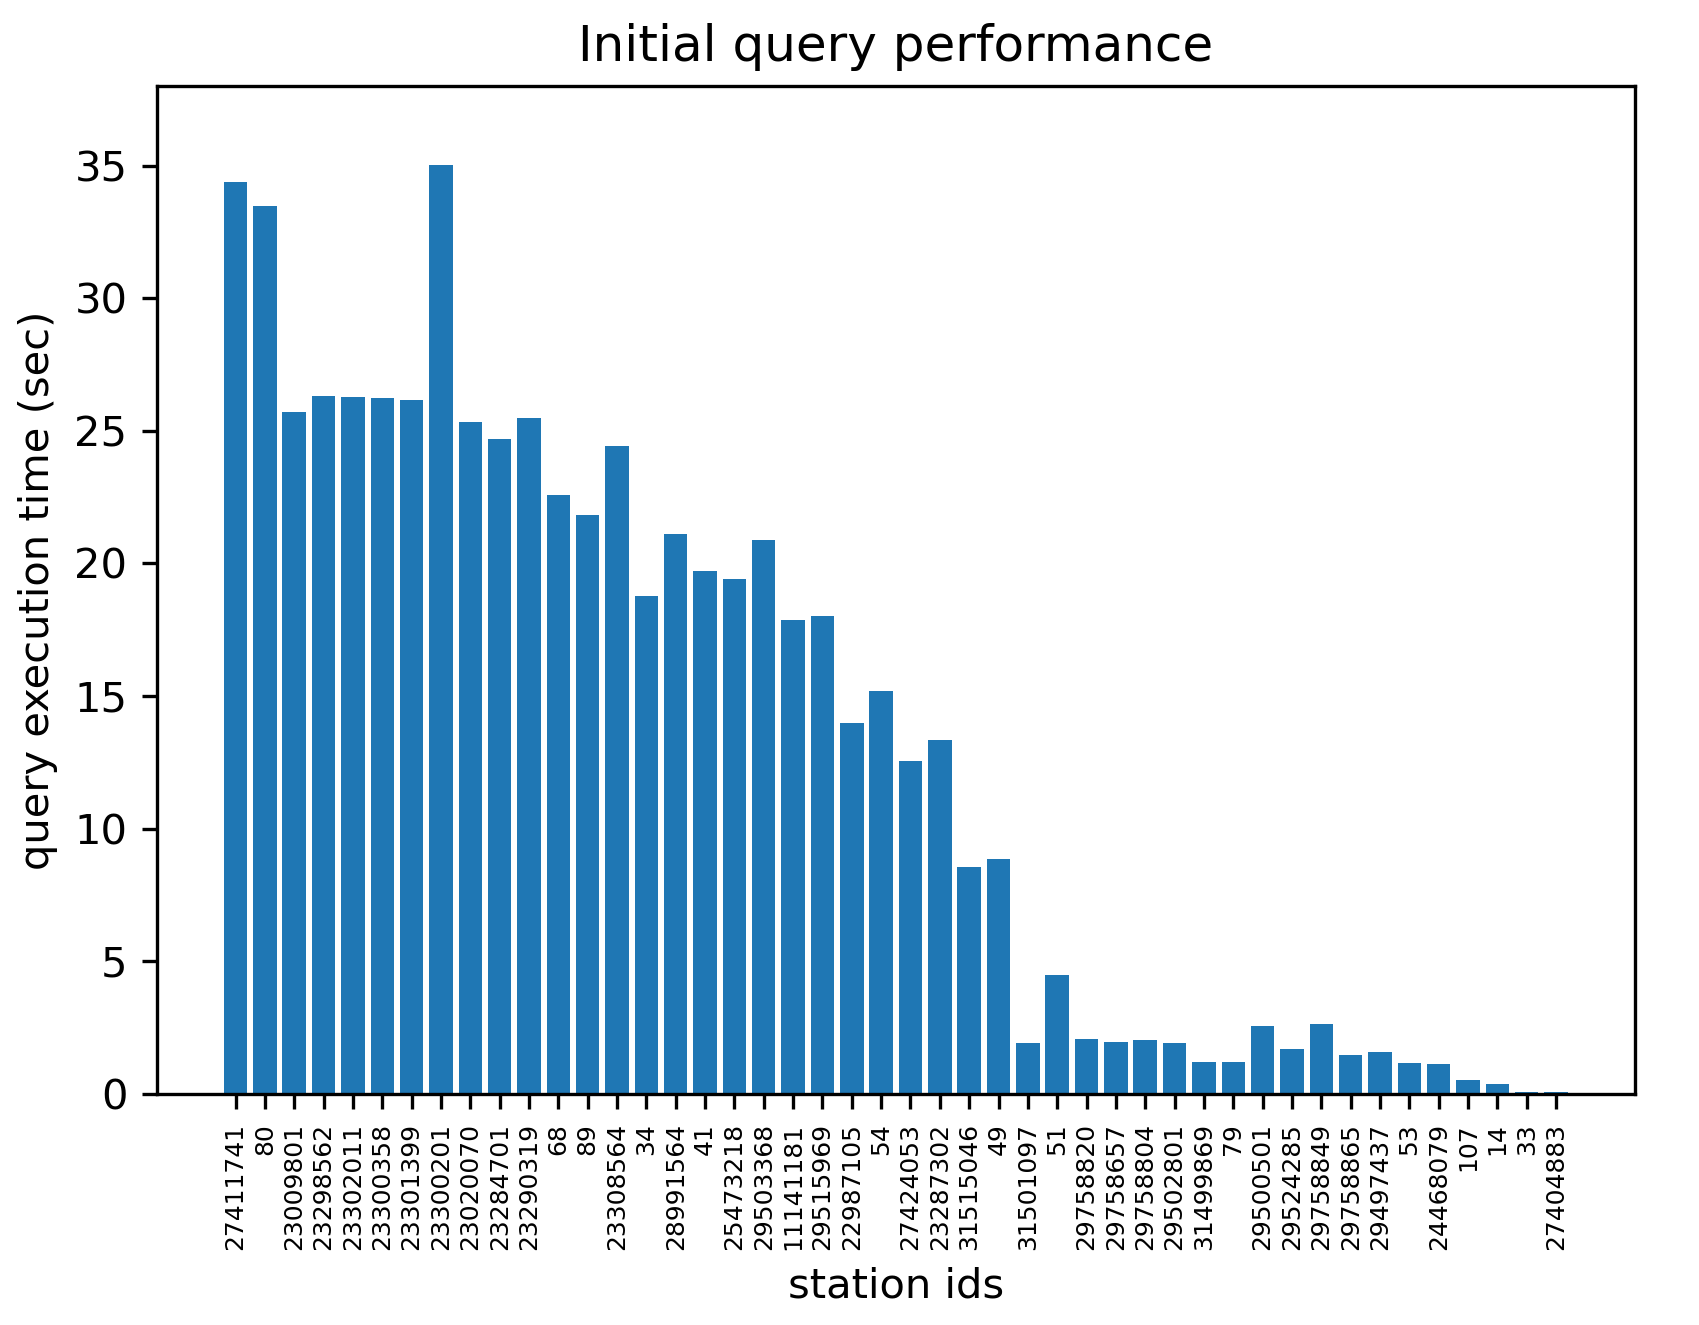
\includegraphics[width=0.85\textwidth,height=\textheight,keepaspectratio]{img/query_prima}
\caption{Tempi di risposta per query temporali sulle centraline AirQino prima dell'ottimizzazione (media su 10 iterazioni)}
\label{fig:query-prima}
\end{figure}

Come si può vedere, per le centraline più attive la query per recuperare la media oraria impiega fino a 35 secondi, un tempo molto elevato.

Per rendere più veloce l'aggregazione dei dati, Timescale mette a disposizione una funzionalità chiamata \textbf{continuous aggregates} (\textit{aggregati continui}).

\subsection{Continuous aggregates}\label{ssec:cont-aggr}
I continuous aggregates sono una funzionalità integrata in TimescaleDB che consente di aggregare i dati in tempo reale, senza la necessità di eseguire query aggiuntive. Funzionano in maniera simile alle viste materializzate di PostgreSQL, con la differenza che non necessitano di essere aggiornati manualmente ogni volta che un nuovo dato viene inserito nella tabella. Infatti, la riaggregazione viene eseguita automaticamente in background tramite una \textbf{refresh policy} definita dall'utente in fase di creazione della vista.

L’utilizzo dei countinuous aggregates offre diversi vantaggi:
\begin{itemize}
  \item Miglioramento delle \textbf{performance}, infatti non è più necessario scansionare tutte le volte la tabella con i dati raw ma è sufficiente leggere questi risultati precalcolati;
  \item Funzionalità avanzate, come la possibilità di salvare i dati raw solo per un periodo di tempo limitato, continuando però a mantenere i dati aggregati. Così facendo si hanno dei dati riassuntivi per eventi che sono molto indietro nel tempo, mentre per gli eventi più recenti si continua ad avere tutti i dati raccolti, portando and un grosso \textbf{risparmio di spazio occupato}.
\end{itemize}

Di contro, lo svantaggio di questa soluzione è che i dati non sono aggiornati ad ogni INSERT effettuata, ma solo ad un intervallo di tempo specificato dall’utente. Questo significa che in fase di lettura i dati più recenti non sono presenti nelle viste materializzate. Per limitare questo problema si potrebbe pensare di diminuire l’intervallo di tempo necessario per il refresh dei dati, ma questo porterebbe ad un aumento del carico computazionale. C'è quindi un compromesso tra la velocità di lettura e l’aggiornamento dei dati. \cite{tesi_polito_2}

Timescale inoltre introduce il concetto di \textit{hypertable}, normali tabelle SQL ma con partizionamento automatico su base temporale.

\subsection{Risultati ottenuti}\label{ssec:cont-aggr-risultati}
Di seguito sono riportati i passi eseguiti sul database di produzione AirQino per l'attivazione del meccanismo di continuous aggregates sulla tabella con i dati dei sensori (\textit{station\_data}):

\begin{enumerate}
  \item  È stato creata la \textit{hypertable} a partire dalla tabella originale, avendo cura di migrare tutti i dati:
\vspace{1mm}
\begin{lstlisting}[language=sql]
SELECT create_hypertable('station_data', 'data_acquired', migrate_data => true);
\end{lstlisting}
Dove \textit{data\_acquired} è la colonna temporale della tabella, in cui vengono salvati data e ora della misurazione.
Questa operazione potrebbe impiegare molto tempo, in base alla quantità di dati nella tabella. Sul database di produzione AirQino ha richiesto circa 36 minuti.
  \item È stato creata la vista materializzata per il calcolo delle medie orarie con continuous aggregates:
\vspace{1mm}
\begin{lstlisting}[language=sql]
CREATE MATERIALIZED VIEW station_data_hourly_avg
WITH (timescaledb.continuous) AS
SELECT time_bucket('1 hour', sd.data_acquired) AS bucket, 
    station_id,  
    sensor_id, 
    avg(sd.float_value) 
FROM station_data sd
GROUP by bucket, station_id, sensor_id;
\end{lstlisting}
Questa operazione sul database di produzione AirQino ha richiesto circa 5 minuti.
  \item Infine, è stata creata una \textit{refresh policy} adeguata:
\vspace{1mm}
\begin{lstlisting}[language=sql]
SELECT add_continuous_aggregate_policy('station_data_hourly_avg',
     start_offset => INTERVAL '7 days',
     end_offset => INTERVAL '1 hour',
     schedule_interval => INTERVAL '1 hour');
\end{lstlisting}
Dove \textit{start\_offset} indica quanto indietro nel tempo vado a calcolare l'aggregato, \textit{end\_offset} indica fino a quando arrivo e schedule indica ogni quanto voglio refreshare la vista.
In questo caso si vanno a refreshare ogni ora i dati della settimana passata (con un'ora di scarto).
Per ragioni di performance conviene sempre escludere l'ultimo bucket (in questo caso l'ultima ora di dati arrivati).
% todo ref
\end{enumerate}

Una volta creata la vista, è possibile ricreare la SELECT originale per la media degli ultimi 7 giorni prendendo i dati da questa nuova tabella di aggregati continui:
\vspace{1mm}
\begin{lstlisting}[language=sql]
SELECT sd.avg
FROM station_data_hourly_avg sd
WHERE bucket > NOW() - INTERVAL '7 days'
AND sd.sensor_id = 29510691 /* id centralina */
ORDER BY bucket DESC;
\end{lstlisting}

Questa nuova query è risultata molto più performante rispetto alla precedente, perchè le medie orarie sono di fatto già precalcolate. I risultati sulle centraline AirQino sono riportati di seguito in figura \ref{fig:query-dopo}.

\begin{figure}[H]
\centering
\captionsetup{justification=centering}
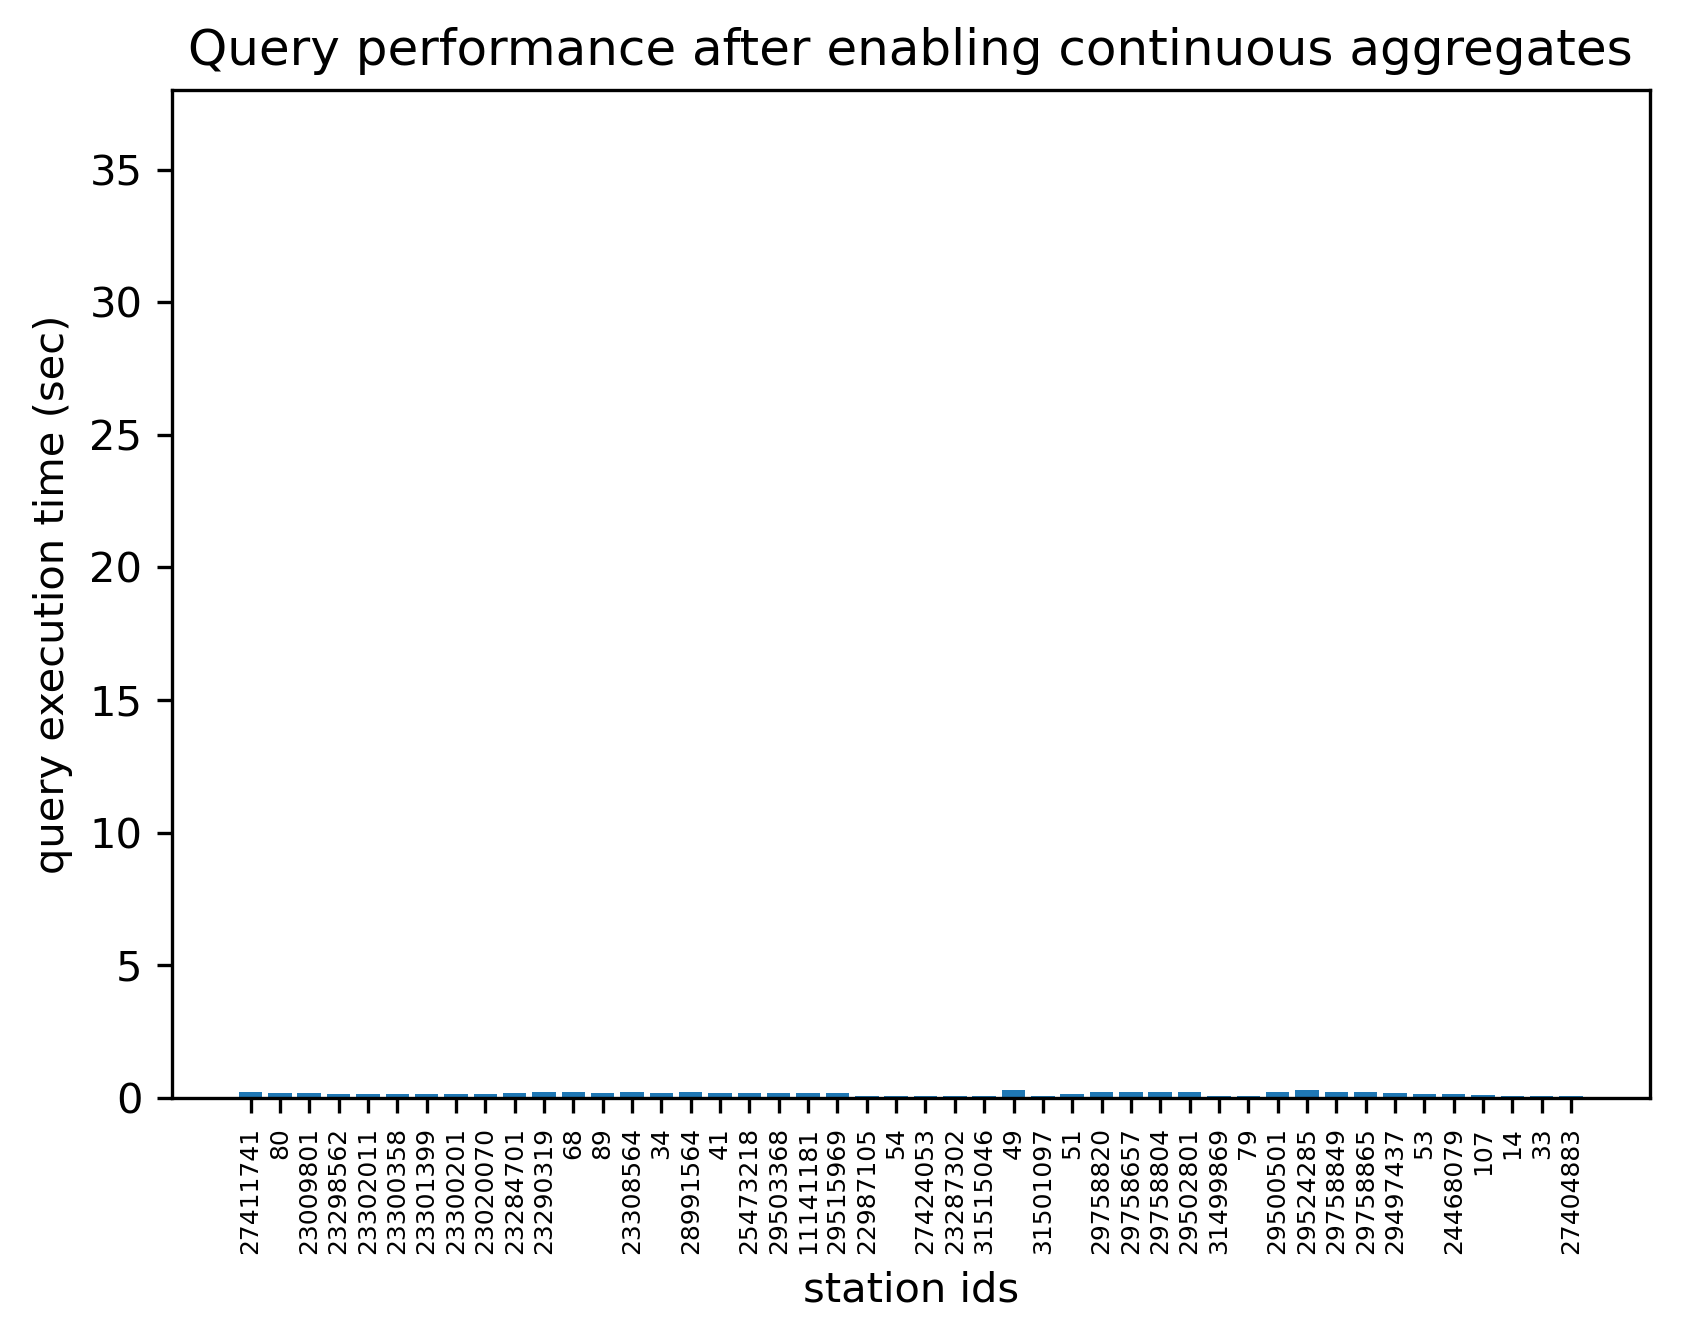
\includegraphics[width=0.85\textwidth,height=\textheight,keepaspectratio]{img/query_dopo}
\caption{Tempi di risposta per query temporali sulle centraline AirQino dopo l'ottimizzazione (media su 10 iterazioni)}
\label{fig:query-dopo}
\end{figure}

Da cui si può notare che con la nuova query, ottimizzata con continuous aggregates, i tempi di risposta risultano costanti per tutte le centraline indipendentemente dalla quantità di dati (con conseguente riduzione significativa dei tempi di risposta, anche 175 volte meno per alcune centraline), garantendo maggiore scalabilità ed efficienza.
